

\section{Continuous Dynamics: Population Gradient Flow}
\label{sec:continuous}

We first analyze the continuous-time population gradient flow dynamics for \eqref{eq:poprisk}, given as
\eq{
\partial_t \bs{W}_t = - \grad R(\bs{W}_t),  ~~ \text{where} ~  \bs{W}_{0} \in \R^{d \times \rs}, ~  \bs{W}_{0,ij} \sim_{iid} \cN \left(0, 1/d \right), \tag{GF} \label{eq:gf} 
}
and the population gradient reads
\eq{
\grad R(\bs{W}_t) =-\frac{1}{2 \sqrt{\rs} \normL} \left( \Th \bs{\Lambda}\Th^\top - \frac{\normL}{\sqrt{\rs}} \W_t \W_t^\top   \right) \W_t.
}
For notational convenience, we write $\mathcal{R}(t) \coloneqq R(\W_t)$ and $\mathcal{A}(t, \bs{\theta}_j) \coloneqq \mathrm{Alignment}(\bs{W}_t, \bs{\theta}_j)$. 
The following theorem sharply characterizes the timescale for alignment and the limiting risk curve. 
For ease of exposition, we drop the prefactor $\frac{1}{8}$ in the population risk so that the population risk starts at $1$.

% \eq{
% \mathcal{R}(t) \coloneqq R(\W_t) ~~ \text{and} ~~ \mathcal{A}(t, \bs{\theta}_j) \coloneqq \mathrm{Alignment}(\bs{W}_t, \bs{\theta}_j).
% }
\begin{theorem}
\label{thm:gfresult}
Let $\lambda_j = j^{-\alpha}$ and $r \asymp d^\beta$ for some $\alpha \geq 0$ and $\beta \in (0,1)$. Consider the regime
\eq{\label{eq:rs-scale}
\begin{cases}
\frac{\rs}{r} \to \varphi \in (0,\infty) \hspace*{-0.5em} & \text{and } ~ d \geq \Omega_{\alpha, \beta, \varphi}(1), \quad  \text{if } \alpha \in [0, 0.5), \\[0.75ex]
\rs \asymp 1,                             & \text{and } ~ d \geq \Omega_{\alpha,\rs}(1), \quad \text{~if } \alpha > 0.5.
\end{cases}  
}
Define the effective student width and effective timescale as
\eq{
r_{\mathrm{eff}} \coloneqq \begin{cases}
\lfloor \rs (1 - \log^{\nicefrac{-1}{8}} \! d) \wedge r \rfloor, & \text{if } \alpha \in [0,0.5) \\
\rs, & \text{if } \alpha > 0.5.
\end{cases} ~~ \text{and} ~~ 
\mathsf{T}_{\mathrm{eff}}   \coloneqq \sqrt{\rs} \norm{\bs{\Lambda}}_\mathrm{F} \log \nicefrac{d}{\rs}.
}
Then, the population \eqref{eq:gf} dynamics satisfy the following   with probability $1 - o(1/d^2) - \Omega(1/\rs^2)$:
\begin{enumerate}[leftmargin = *, itemsep=0mm]
    \item \textbf{Alignment:} For $j \leq r_{\mathrm{eff}}$  and $t > 0$ satisfying $t \asymp r^\alpha$ when $\alpha  \in [0,0.5)$ and $t \asymp 1$ when $\alpha > 0.5$, we have
        \eq{
            \mathcal{A}  \big(t  \mathsf{T}_{\mathrm{eff}}, \bs{\theta}_j \big) = \mathbbm{1}\{t \geq  \tfrac{1}{\lambda_j} \} + o_d(1). \label{eq:GF-alignment}
        }
    \item  \textbf{Risk curve:} Under the same time scaling,  
        \eq{
        \mathcal{R} \big(t  \mathsf{T}_{\mathrm{eff}} \big) = 1 -\frac{1}{\normL^2} \sum_{j = 1}^{r_{\mathrm{eff}}} \lambda_j^2   \mathbbm{1}\{t  \geq \tfrac{1}{\lambda_j}\}    + o_d(1). \label{eq:GF-risk}
        }
\end{enumerate}
\end{theorem}



\begin{remark}
We make the following remarks about our result in Theorem \ref{thm:gfresult}:
\begin{itemize}[leftmargin=*]
\item  The spectral decay rate $\alpha$ determines both the choice of student width $\rs$ and the timescale needed for learning in Theorem \ref{thm:gfresult}. Specifically, when $\alpha > 1/2$ (i.e., light-tailed regime), the target coefficients $\{ \lambda_j \}_{j = 1}^r$ are square-summable, making the teacher model effectively finite-dimensional. Therefore, a finite-width student suffices, and only finitely many directions need to be learned to achieve small loss, which results in a timescale of order $\log d$. In contrast, for the heavy-tailed regime $\alpha < 1/2$, we need to recover linear-in-$r$ directions to achieve small population loss, which require both proportional width $r_s / r \to \varphi$ and a longer timescale $r \log d$. 
This difference in timescale will be made explicit in Corollary~\ref{cor:asympriskcont}. 
\item Theorem \ref{thm:gfresult} verifies the \textit{additive model} hypothesis \cite{michaud2024quantization} for quadratic neural networks in the feature learning regime; specifically, \eqref{eq:GF-alignment} identifies sharp transition time in alignment between student weights and the $j$-th teacher direction, and \eqref{eq:GF-risk} suggests that the cumulative loss can be decomposed into individual emergent risk curves where the timescale is decided by the signal strength $\lambda_j$. 
\end{itemize}

\end{remark}



\paragraph{Neural scaling laws.}
As a corollary of Theorem \ref{thm:gfresult}, we obtain the following risk characterization.
\begin{corollary}
\label{cor:asympriskcont}
By Theorem \ref{thm:gfresult}, the asymptotic risk of \eqref{eq:gf} is given as follows: 
\begin{itemize}[leftmargin = *, itemsep=0mm]
    \item   Heavy-tailed regime ($\alpha \in [0,0.5)$): Almost surely, for all $t > 0$
    $$\mathcal{R}(t r \log d)
    \xrightarrow
    {d \to \infty}
    %\mathcal{R}_{\text{heavy}}(\tau) = 
    \big(1 - C t^{\frac{1 - 2 \alpha}{\alpha}}  \big)_+  \vee \big(1 - \varphi^{1 - 2\alpha}\big)_+.$$ 
    % where $C$ is an $(\alpha,\beta)$-dependent constant.  
    \item Light-tailed regime ($\alpha > 0.5$):  With probability  $1 - \Omega(1/\rs)$, for all $t > 0$, the risk $\mathcal{R}(t \log d)$ converges as $d \to \infty$ to a deterministic limit satisfying
    \eq{
    \mathcal{R}(t \log d) \xrightarrow{d \to \infty}
    \Theta\left( t^{- \frac{2\alpha - 1}{\alpha}} + \rs^{-(2\alpha - 1)} \right).
    }
    % where $C$ is an $\alpha$-dependent constant.
\end{itemize}
\end{corollary}
Corollary \ref{cor:asympriskcont} shows that, over appropriate timescales, the cumulative effect of these emergent transitions yields a smoothly decaying risk curve. Intuitively speaking, the power-law exponent arises from the Riemann integral approximation of the infinite sum \eqref{eq:GF-risk} -- see Appendix~\ref{app:scaling-proof} for details. 

The asymptotic risk behavior in Corollary \ref{cor:asympriskcont} is visualized in Figure \ref{fig:asymptoticriskgf}  (see also Figure~\ref{fig:intro}(b) for empirical simulation). The figure illustrates how the sharp, step-like emergent curve at $\alpha = 0$ (as observed in earlier works on multi-index learning \cite{benarous2021online,abbe2023sgd}) gradually transitions into a smooth curve as $\alpha$ increases. Notably, in the light-tailed regime $\alpha>1/2$, our risk curve resembles the neural scaling laws in \cite{kaplan2020scaling,hoffmann2022training} which takes the form of $\cR \sim 1/(\text{Data size})^a + 1/(\text{Model size})^{b}$, where the data size can be connected to optimization time under the one-pass discretization, which we analyze in the ensuing section. 


\begin{figure}[t]
% \vspace{-5mm}
    \centering
    \begin{subfigure}[t]{0.56\textwidth}
        \centering
        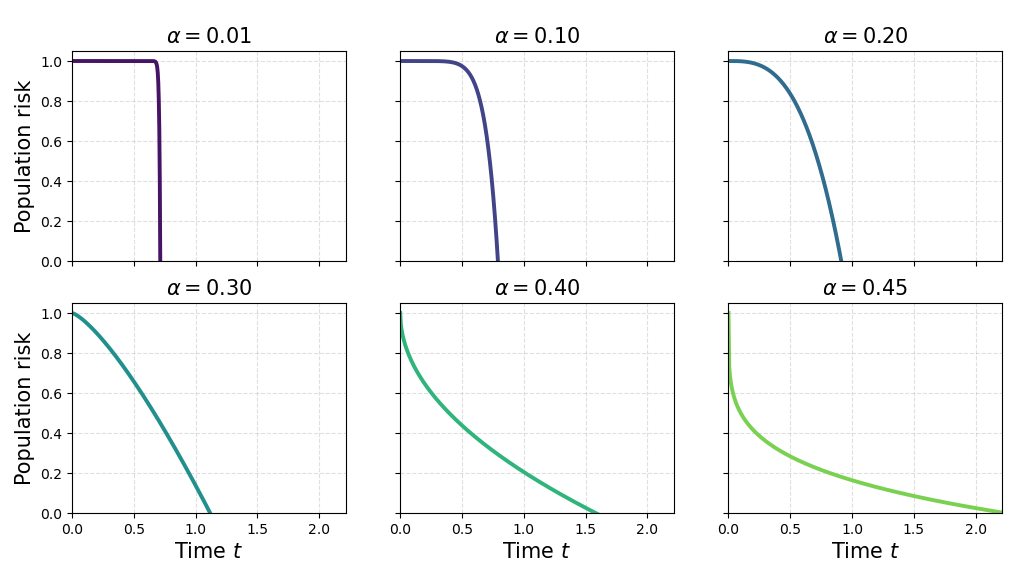
\includegraphics[width=\textwidth]{_figures/heavy_tailed_gf.png}
        \caption{Heavy-tailed regime $(\alpha<1/2)$.}
    \end{subfigure} 
    \begin{subfigure}[t]{0.345\textwidth}
        \centering
        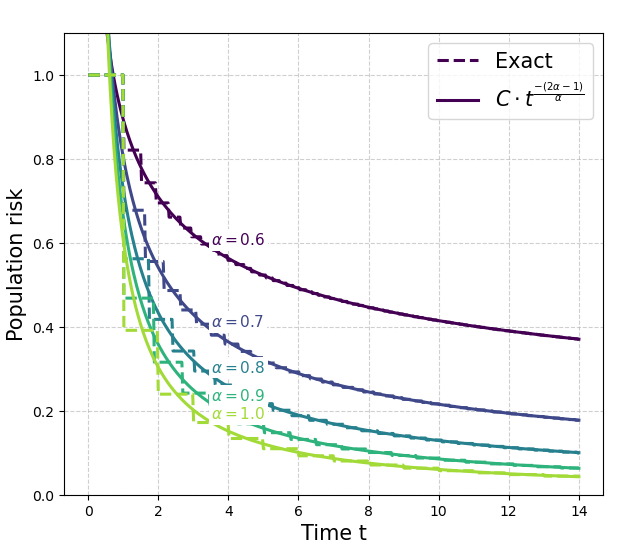
\includegraphics[width=\textwidth]{_figures/light_tailed_gf.png}
        \caption{Light-tailed regime $(\alpha>1/2)$.}
    \end{subfigure}
    \caption{\small Illustration of the limiting risk trajectories and scaling behavior given in Corollary \ref{cor:asympriskcont}.}
    \label{fig:asymptoticriskgf}
    % \vspace{-0.5mm}
\end{figure}




\section{Discrete Dynamics: Online Stochastic Gradient Descent}
\label{sec:discrete}
% \vspace{-1mm}
Now we analyze the finite-sample, discrete-time counterpart of the population dynamics \eqref{eq:gf} and establish computational and statistical guarantees. 
We first discretize the directional component of the dynamics via online SGD with Stiefel constraint (see Proposition \ref{prop:sgdrotation}), and then introduce a fine-tuning step with negligible statistical and computational cost to fit the radial component; this mirrors the layer-wise training paradigm commonly used in theoretical analyses of gradient-based feature learning \cite{abbe2022merged,damian2022neural,ba2022high,barak2022hidden}.  
The procedure is summarized in Algorithm~\ref{alg:sgd}.  

\vspace{-1.mm} 

  
\begin{algorithm}[H]
\caption{Online Stochastic Gradient Descent (Stiefel)
\label{alg:sgd}}
\begin{algorithmic}[1] 
\setlength{\itemsep}{0.25ex}
\For{$t = 1,2, \dots$}
    \State $\bs{\widetilde{W}}_{t} = \bs{W}_{t-1} - \eta \nabla_{\mathrm{St}} \mathcal{L}(\bs{W}_{t-1})$  
    \State $\bs{W}_{t} = \bs{\widetilde{W}}_{t} \left( \bs{\widetilde{W}}_{t}^\top \bs{\widetilde{W}}_{t} \right)^{-1/2}$ \Comment{Feature learning}
\EndFor \vspace{0.4em}
\State \label{line:finetuning} $\bs{W}^{\mathrm{final}}_{t} \! = \! \bs{W}_t \bs{\Omega}_*$  where $ \bs{\Omega}_* =  {\displaystyle \argmin_{\bs{\Omega}  \in \R^{\rs \times \rs}} } \sum_{j = 1}^{N_{\mathrm{Ft}}} \mathcal{L}\big(\W_t \bs{\Omega}; (\bs{x}_{t+j}, y_{t+j}) \big)$ \Comment{Fine-tuning}
\end{algorithmic}  
\end{algorithm}
\vspace{-2mm}

In the feature learning step, we update the first-layer weights $\W_t$ to recover the subspace spanned by the teacher directions. To this end, we use online SGD on Stiefel manifold~\cite{arous2024high} with polar retraction.  The Riemannian gradient on the Stiefel manifold is given by:
\eq{\textstyle
\nabla_{\mathrm{St}} \mathcal{L}(\bs{W}_{t-1}) & \coloneqq \nabla  \mathcal{L}(\textstyle\bs{W}_{t-1})- \frac{1}{2}  \bs{W}_{t-1} \left( \bs{W}_{t-1}^\top  \nabla  \mathcal{L}(\bs{W}_{t-1}) + \nabla  \mathcal{L}(\bs{W}_{t-1})^\top  \bs{W}_{t-1}  \right), 
}
where the instantaneous loss is defined for  the sample $(\bs{x}_{t}, y_{t})$.
Since the goal is to ensure subspace alignment as in \eqref{def:alignment}, the overlap of individual student-teacher weights is not relevant during this phase.

After the feature learning phase, we perform a fine-tuning step to rotate $\bs{W}_t$ so that each $\bs{w}_j$ aligns with the corresponding teacher direction $\bs{\theta}_j$. This is achieved by solving an empirical risk minimization problem over $N_{\mathrm{Ft}}$ fresh samples.  The optimal fine-tuning matrix $\bs{\Omega}_*$ admits a closed-form solution that is also numerically easy to compute. Importantly, the computational and statistical complexity of this step scales only quadratically with the student width $\rs$, which is negligible compared to the cost of feature learning. 
The derivation and complexity analysis for this phase are provided in Appendix~\ref{sec:finetuning}.

\begin{remark}
Recall that the stage-wise training procedure is not required in our continuous-time analysis in Section~\ref{sec:continuous}. This is because we employ a Stiefel gradient similar to \cite{bietti2023learning,arous2024high} -- which alone cannot fit the radial component -- to simplify the discretization analysis. 
We conjecture that a standard Euclidean discretization of \eqref{eq:gf} can also achieve the same risk scaling; see Figure~\ref{fig:intro}(b) for empirical evidence. 
\end{remark}



We define the population risk of the output of Algorithm~\ref{alg:sgd}, the alignment with a teacher direction $\bs{\theta}_j$, and the optimal risk achievable by a student neural network with width $\rs$ respectively as
\eq{\textstyle
\mathcal{R}(t) \coloneqq R(\W_t^{\mathrm{final}}), \quad
\mathcal{A}(t, \bs{\theta}_j) \coloneqq \mathrm{Alignment}(\bs{W}_t, \bs{\theta}_j), \quad
\mathcal{R}_{\mathrm{opt}} \coloneqq \frac{1}{\normL^2} \sum_{j = (\rs \wedge r) + 1}^{r} \lambda_j^2.
}
Intuitively, $\cR_{\mathrm{opt}}$ is the risk achieved by exactly fitting the top $r_s\le r$ components of the teacher model. 
Note that the alignment $\mathcal{A}(t, \bs{\theta}_j)$ depends only on the directional component of $\bs{W}_t$; thus, this quantity remains unchanged during fine-tuning. 
The following theorem characterizes the alignment and risk curve for the discrete-time Algorithm~\ref{alg:sgd}.
 
 
\begin{theorem}
\label{thm:sgdresult}
Let the parameters $\{\lambda_j\}_{j=1}^r$, $r$,$r_s$, $r_{\mathrm{eff}}$ and $\mathsf{T}_{\mathrm{eff}}$,
and the scaling regime~\eqref{eq:rs-scale}
be as in Theorem~\ref{thm:gfresult}.
Suppose the student weights are initialized uniformly on the Stiefel manifold, and that the step size $\eta$ and fine-tuning sample size  $N_{\mathrm{Ft}}$ satisfy
\eq{
\eta  \asymp \frac{1}{d} \begin{cases}
\frac{1}{r^{\alpha} \log^{C_{\alpha}} (1 + d/\rs)}, & \alpha \in [0,0.5) \\[0.3em] 
\frac{1}{\log^{C_{\alpha}} \! d}, & \alpha > 0.5    
\end{cases}  ~~ \text{and} ~~ N_{\textrm{Ft}} \asymp \rs^2 \log^5 d,
}
for some constant $C_\alpha > 0$ depending only on $\alpha$.
Then with probability $1 - o_d(1/d^2) - \Omega(1/\rs^2)$, 
\begin{enumerate}[leftmargin = *]
    \item \textbf{Runtime and sample complexity:} If 
    \eq{
    T \geq  \begin{cases}
        d r^{1+\alpha} \log^{C_{\alpha} +1}(1 + d/\rs), & \alpha \in [0,0.5) \\
        d \log^{C_{\alpha} +1} d, & \alpha > 0.5.
    \end{cases} \label{eq:samplecomplexity}
    }
    we have
    $
    \mathcal{R}(T) =  \mathcal{R}_{\mathrm{opt}} + o_d(1).
    $
    \item \textbf{Alignment and Risk curve:} For $t > 0$ satisfying $t \asymp r^\alpha/\eta$ when $\alpha  \in [0,0.5)$ and $ t \asymp 1/\eta$ when $\alpha > 0.5$, 
    \[
    \bullet~ \mathcal{A}\big(t \mathsf{T}_{\mathrm{eff}}, \bs{\theta}_j\big) 
    = \mathbbm{1}\{ \eta t \geq \tfrac{1}{\lambda_j}\} + o_d(1)   \text{~for~} j \leq r_{\mathrm{eff}}.
     \quad\bullet~ \mathcal{R}\big(t \mathsf{T}_{\mathrm{eff}}\big) 
    = 1 - \frac{1}{\normL^2} \sum_{j = 1}^{r_{\mathrm{eff}}} \lambda_j^2 \, \mathbbm{1}\{ \eta t \geq \tfrac{1}{\lambda_j} \} + o_d(1). 
    \]
\end{enumerate}
\end{theorem}
\begin{remark}
We make the following remarks on the sample complexity. 
\begin{itemize}[leftmargin=*]
    \item The bound in \eqref{eq:samplecomplexity} implies a complexity of  $n\asymp T \! \simeq \!  d r^{1+\alpha} \, \mathrm{polylog}(1 + d / r_s)$  in the heavy-tailed case, and $T \simeq d \, \mathrm{polylog}(d)$ in the light-tailed case. Note that due to the one-pass nature of the algorithm, the runtime and sample complexity are identical (up to the negligible fine-tuning step). 
    \item In the light-tailed regime ($\alpha > 1/2$), the required sample size $n \simeq d \, \mathrm{polylog}(d)$ is information theoretically optimal up to logarithmic factors. Note that kernel methods and neural networks in the lazy regime \cite{jacot2018neural,chizat2018note} requires $n\gtrsim d^2$ samples to learn a quadratic target function; thus our sample complexity bound illustrates the benefit of feature learning. 
    \item In the heavy-tailed regime ($\alpha<1/2$), we obtain (nearly) information theoretically optimal sample complexity when $\alpha=0$ (see discussion below). For the intermediate regime $\alpha\in (0,1/2)$, we conjecture that the optimal sample complexity is $T \simeq d r$, which implies our current bound is suboptimal by a factor of $r^{\alpha}$. 
\end{itemize}
\end{remark}

\paragraph{Isotropic Setting $(\alpha=0)$.} 
In the isotropic case, where the goal is to estimate the $r$-dimensional subspace spanned by the teacher weights, the above theorem yields a sample and runtime complexity $n\asymp T \asymp d r \, \mathrm{polylog}(1 + d / r_s)$. This interpolates between the $n \simeq d \, \mathrm{polylog}(d)$ rate for phase retrieval $r = 1$~\cite{tan2019online,benarous2021online}, and $n \simeq d^2$  as $r \to d$, which matches the sample complexity in the linear-width regime \cite{maillard2024bayes,erba2025nuclear}. 
Notably, our $r$-dependence improves upon the recent work of \cite{ren2024learning}, which established a sufficient sample size of $n \gtrsim d \, \mathrm{poly}(r)$ for a similar quadratic setting.  
We expect our result to be optimal up to polylogarithmic factors due to the intrinsic $dr$-dimensional nature of the subspace recovery problem.


\paragraph{Scaling laws in discrete time.} As indicated by the alignment and risk expressions in Theorem~\ref{thm:sgdresult}, a sufficiently small learning rate $\eta$ ensures that running online SGD for $t$ steps closely tracks the population gradient flow trajectory \eqref{eq:gf} at time $\eta t$, exhibiting the same scaling behavior. The following corollary formalizes the discrete-time counterpart of Corollary~\ref{cor:asympriskcont}.


\begin{corollary}
\label{cor:asympriskdis}
By Theorem \ref{thm:sgdresult}, the asymptotic risk of Online SGD is given as follows:
\begin{itemize}[leftmargin = *,noitemsep]
    \item   Heavy-tailed case ($\alpha \in [0,0.5)$): Almost surely, for all $t > 0$
    $$\mathcal{R}(t r \log d)
    \xrightarrow
    {d \to \infty}
    %\mathcal{R}_{\text{heavy}}(\tau) = 
    \big(1 - C (\eta t)^{\frac{1 - 2 \alpha}{\alpha}}  \big)  \vee (1 - \varphi^{1 - 2\alpha})_+.$$ 
    \item Light-tailed case ($\alpha > 0.5$): With probability  $1 - \Omega(1/\rs)$, for all $t > 0$, the risk $\mathcal{R}(t \log d)$ converges as $d \to \infty$ to a deterministic limit satisfying
    $$\mathcal{R}(t \log d)
    \xrightarrow{d \to \infty}
    \Theta  \big(   (\eta t)^{- \frac{2 \alpha - 1}{\alpha}} + \rs^{- (2 \alpha  - 1)}  \big).$$
\end{itemize}
\end{corollary}
 


